% !TeX spellcheck = fr_FR
\chapter{Chapitre 2 : Transport public dans OSM}

La cartographie du transport public dans OpenStreetMap (OSM) a évolué à travers plusieurs schémas. Cette évolution a conduit à la coexistence de diverses combinaisons de balises pour les arrêts de bus, gares ferroviaires, stations de tramway et autres nœuds de transport. De plus, comme OSM est un projet maintenu par une communauté de volontaires, certaines entrées peuvent ne correspondre à aucun schéma précis.

Dans cette section, nous analysons les différents schémas existants, nous présentons la requête utilisée (c’est-à-dire quelles données seront extraites) et, une fois les données obtenues, nous proposons une vue d’ensemble de l’usage des balises pour les nœuds d’arrêts de transport public dans OSM en Suisse.

\medskip
\noindent\textbf{Reproductibilité.} Les figures et statistiques de ce chapitre sont produites par des scripts sous \texttt{memoire/scripts\_used/chap2/}. Le script principal est \texttt{osm\_plots.py} et lit \texttt{data/raw/osm\_data.xml} ainsi que les fichiers traités générés par \texttt{get\_osm\_data.py}.

\section{Schémas de cartographie du transport public dans OSM}
\begin{itemize}
    \item \textbf{Schéma d'origine (PTv1)} : La méthode la plus ancienne et encore très répandue, qui attribue à chaque arrêt des balises spécifiques au mode concerné. Par exemple, un arrêt de bus est simplement \texttt{highway=bus\_stop} [\ref{ref:osm_bus_stop}], une gare ferroviaire est \texttt{railway=station} (ou \texttt{railway=halt} pour des arrêts plus petits), et un arrêt de tramway est \texttt{railway=tram\_stop}. Ces balises figurent souvent sur un seul nœud représentant l'emplacement où les passagers attendent.
    PTv1 est largement utilisé encore aujourd’hui [\ref{ref:osm_public_transport}].
    Il est important de noter qu’aucune de ces balises héritées n’a été formellement dépréciée par les propositions plus récentes, ce qui explique qu’elles restent toujours en usage actif.

    \item \textbf{Schéma Oxomoa (années 2010)} : Schéma intermédiaire développé vers 2010 (par l’utilisateur Oxomoa), il introduisait une structure plus aboutie, ressemblant à ce que PTv2 allait proposer plus tard. Ce schéma utilisait des relations de type ``route'' et des relations de type ``stop area'' pour regrouper les éléments d’arrêt [\ref{ref:osm_public_transport}]. Bien qu’il ait influencé la version suivante, ce schéma est désormais historique, même si certains itinéraires plus anciens ($\sim$2010) le suivent encore.

    \item \textbf{Nouveau schéma de transport public (PTv2)} : Approuvé en 2011, PTv2 a introduit un système de balisage plus puissant mais plus complexe [\ref{ref:osm_proposal_public_transport}]. L’idée est de séparer la notion d’arrêt en stop positions (là où le véhicule s’arrête sur la chaussée ou la voie) et platforms (où les passagers attendent). Dans ce schéma, un arrêt de bus est généralement représenté par \textit{deux} objets reliés :
    \begin{itemize}
        \item un nœud sur la chaussée avec \texttt{public\_transport=stop\_position} (souvent accompagné de \texttt{bus=yes} ou \texttt{tram=yes}, etc., pour préciser le mode) [\ref{ref:osm_key_public_transport}],
        \item et un nœud (ou une zone) en bord de route portant la balise \texttt{public\_transport=platform} (en plus d’une balise pour le mode ou d’une balise héritée).
    \end{itemize}
    
    Par exemple, un nœud de plate-forme de bus peut porter \texttt{public\_transport=platform + bus=yes}, tandis que le nœud correspondant sur la chaussée sera \texttt{public\_transport=stop\_position + bus=yes} [\ref{ref:osm_key_public_transport}]. En pratique, les cartographes incluent souvent l’ancienne balise sur l’un de ces objets pour assurer la compatibilité – par exemple, on retrouvera \texttt{highway=bus\_stop} sur le nœud de la plate-forme, afin qu’il soit reconnu par les outils traditionnels [\ref{ref:osm_bus_stop}].
    
    PTv2 introduit également la notion de relation stop\_area (\texttt{type=public\_transport + public\_transport=stop\_area}) pour regrouper tous les éléments d’une même station ou d’un même arrêt, et une relation route\_master pour regrouper les itinéraires dans les deux sens [\ref{ref:osm_proposal_public_transport}]. Fait notable, la proposition PTv2 n’a pas invalidé ni remplacé les balises existantes, ce qui signifie que les balises PTv1 (telles que \texttt{highway=bus\_stop}, \texttt{railway=station}) coexistent souvent avec les balises PTv2 pour un même arrêt [\ref{ref:osm_public_transport}]. De nombreuses communautés encouragent à ajouter les balises PTv2 tout en conservant les anciennes pour plus de complétude.
\end{itemize}


\noindent\textit{Remarque (zones).} Pour ce projet, nous ne considérons ici que les \textbf{nœuds}. Par simplification, les \textit{plateforms} ou \textit{stop\_positions} modélisés comme \textbf{zones} (ways/relations) ne sont pas intégrés au comptage. Il peut exister des \texttt{public\_transport=platform} ou \texttt{public\_transport=stop\_position} cartographiés en zones.


\section{Différences dans l’usage de clés spécifiques}
Certains choix de clés varient parmi les cartographes, ce qui peut engendrer des divergences dans la manière de consigner l'information :

\begin{itemize}
    \item \texttt{ref} vs \texttt{local\_ref} (codes d'arrêt) : De nombreux arrêts de transport public possèdent un code ou identifiant officiel (numéro ou lettre fourni par l'autorité de transport). Les cartographes utilisent tantôt la balise générique \texttt{ref=}, tantôt \texttt{local\_ref=}. La recommandation OSM est : utiliser \texttt{ref=} pour le code d'arrêt à l'échelle du réseau (un ID unique dans le système de transport) et \texttt{local\_ref} si c'est un code/lettre propre à un contexte plus restreint [\ref{ref:osm_local_ref}].
    
    Par exemple, un arrêt de bus qui a l'ID ``3154'' dans la base de la ville se balisera \texttt{ref=3154}. Et si cet arrêt comporte plusieurs quais, nommés ``Bay C'' par exemple, on peut utiliser \texttt{local\_ref=C} sur le quai concerné. En pratique, la distinction n’est pas toujours respectée : certains mettent tous les codes dans \texttt{ref}, d’autres utilisent \texttt{local\_ref} pour les numéros de quai ou les lettres d’arrêt.
\end{itemize}

\section{Requête Overpass transport public — Suisse}
Overpass est un système de requêtage permettant d'extraire des données depuis la base de données OpenStreetMap [\ref{ref:overpass_turbo}]. Il utilise un langage de requête appelé Overpass Query Language, qui permet de rechercher et filtrer des objets OSM (nœuds, chemins, relations) en fonction de critères spécifiques (tags, zones géographiques, types d'objets, etc.).
Pour obtenir les arrêts de transport public en Suisse sur OpenStreetMap, nous utilisons la requête Overpass suivante (simplifiée et \textit{dédoublonnée}) :

\begin{tcolorbox}[colback=gray!10, colframe=brown, title=Requête Overpass]
\begin{verbatim}
[out:xml][timeout:180];
area["ISO3166-1"="CH"]->.searchArea;
(
  node(area.searchArea)["public_transport"~"platform|stop_position"];
  node(area.searchArea)["highway"="bus_stop"];
  node(area.searchArea)["railway"~"station|halt|tram_stop"];
  node(area.searchArea)["amenity"~"bus_station|ferry_terminal"];
  node(area.searchArea)["aerialway"="station"];
);
out;
relation(bn)[type=route];
out meta;
\end{verbatim}
\end{tcolorbox}

Cette requête commence par définir la zone d’intérêt, qui correspond à la Suisse, identifiée par le code ISO3166-1 \texttt{CH}. Ensuite, elle sélectionne différents types de nœuds correspondant aux infrastructures de transport public. Cette requête inclut des arrêts de bus et de tram, des terminaux de ferries, des stations de remontées mécaniques, etc.


Enfin, la requête extrait également les relations de type \texttt{route} associées aux nœuds obtenus. Cette information est pertinente, car elle permet de lier les arrêts à leurs itinéraires respectifs, ce qui facilitera les correspondances avec d’autres sources de données, comme les données ATLAS.

\section{Aperçu des balises (\textit{tags}) des nœuds OSM en Suisse}
Une fois les nœuds obtenus par la requête ci-dessus, nous analysons les balises présentes sur ces nœuds.\
Nous montrons d’abord quelques exemples :
\begin{tcolorbox}[colback=gray!10, colframe=brown, title=OSM N\oe ud : Grand-Mont]
\begin{verbatim}
<node id="2368323780" lat="46.5627599" lon="6.6343369">
   <tag k="bus" v="yes"/>
   <tag k="highway" v="bus_stop"/>
   <tag k="local_ref" v="D"/>
   <tag k="name" v="Grand-Mont"/>
   <tag k="network" v="Mobilis"/>
   <tag k="operator" v="TL"/>
   <tag k="public_transport" v="stop_position"/>
   <tag k="tactile_paving" v="no"/>
   <tag k="trolleybus" v="yes"/>
   <tag k="uic_name" v="Le Mont-sur-L., Grand-Mont"/>
   <tag k="uic_ref" v="8504177"/>
 </node>
\end{verbatim}
\end{tcolorbox}
\begin{tcolorbox}[colback=gray!10, colframe=brown, title=OSM N\oe ud sans nom]
\begin{verbatim}
<node id="2368860496" lat="46.4418646" lon="6.9764107">
   <tag k="aerialway" v="station"/>
 </node>
\end{verbatim}
\end{tcolorbox}
\begin{tcolorbox}[colback=gray!10, colframe=brown, title=OSM N\oe ud : Interlaken Ost]
\begin{verbatim}
</node>
 <node id="2388274179" lat="46.6910098" lon="7.8697428">
   <tag k="name" v="Interlaken Ost"/>
   <tag k="public_transport" v="stop_position"/>
   <tag k="railway" v="stop"/>
   <tag k="ref" v="7"/>
   <tag k="train" v="yes"/>
 </node>
\end{verbatim}
\end{tcolorbox}

Comme on le voit, chaque nœud contient des balises différentes. Voici quelques statistiques pour une vision générale (sur notre extraction) :
\begin{itemize}
    \item Nombre total de nœuds : 60 635
    \item Nombre total de nœuds avec \texttt{public\_transport} == \texttt{platform} : 24 548
    \begin{itemize}
        \item Parmi ceux-ci avec \texttt{uic\_ref} : 22 986
        \item Nœuds de plateforme avec une position d'arrêt correspondante (même \texttt{uic\_ref}) : 13 571
        \item Nœuds de plateforme avec \texttt{uic\_ref} mais sans position d'arrêt correspondante : 9 415
    \end{itemize}
    \item Nombre total de nœuds avec \texttt{public\_transport} == \texttt{stop\_position} : 30 018
    \begin{itemize}
        \item Parmi ceux-ci avec \texttt{uic\_ref} : 28 199
    \end{itemize}
    \item Nœuds avec toutes les balises (\texttt{uic\_ref}, \texttt{local\_ref}, \texttt{name}, \texttt{network}, \texttt{operator}, \texttt{uic\_name}) : 3 875
    \item Nœuds avec \texttt{uic\_ref} : 55 166
    \begin{itemize}
        \item Parmi ceux-ci, avec \texttt{ref} : 2 796
        \item Parmi ceux-ci, avec \texttt{local\_ref} : 4 314
        \item Parmi ceux-ci, avec \texttt{ref} et \texttt{local\_ref} : 307
        \item Parmi ceux-ci avec \texttt{name} : 55 147
        \item Parmi ceux-ci avec \texttt{network} : 40 576
        \item Parmi ceux-ci avec \texttt{operator} : 53 322
        \item Parmi ceux-ci avec \texttt{uic\_name} : 55 042
    \end{itemize}
    \item Nœuds sans \texttt{uic\_ref} : 5 469
    \begin{itemize}
        \item Parmi ceux-ci, avec \texttt{ref} : 200
        \item Parmi ceux-ci, avec \texttt{local\_ref} : 288
        \item Parmi ceux-ci, avec \texttt{ref} et \texttt{local\_ref} : 13
        \item Parmi ceux-ci avec \texttt{name} : 4 339
        \item Parmi ceux-ci avec \texttt{network} : 758
        \item Parmi ceux-ci avec \texttt{operator} : 1 542
        \item Parmi ceux-ci avec \texttt{uic\_name} : 86
    \end{itemize}
    \item Nombre total de nœuds sans aucune des balises \texttt{uic\_ref}, \texttt{ref}, \texttt{local\_ref}, \texttt{network}, \texttt{operator}, \texttt{uic\_name} : 1 084
    \item Nœuds non assignés avec \texttt{aerialway=station} : 817
\end{itemize}

\begin{figure}[H]
  \centering
  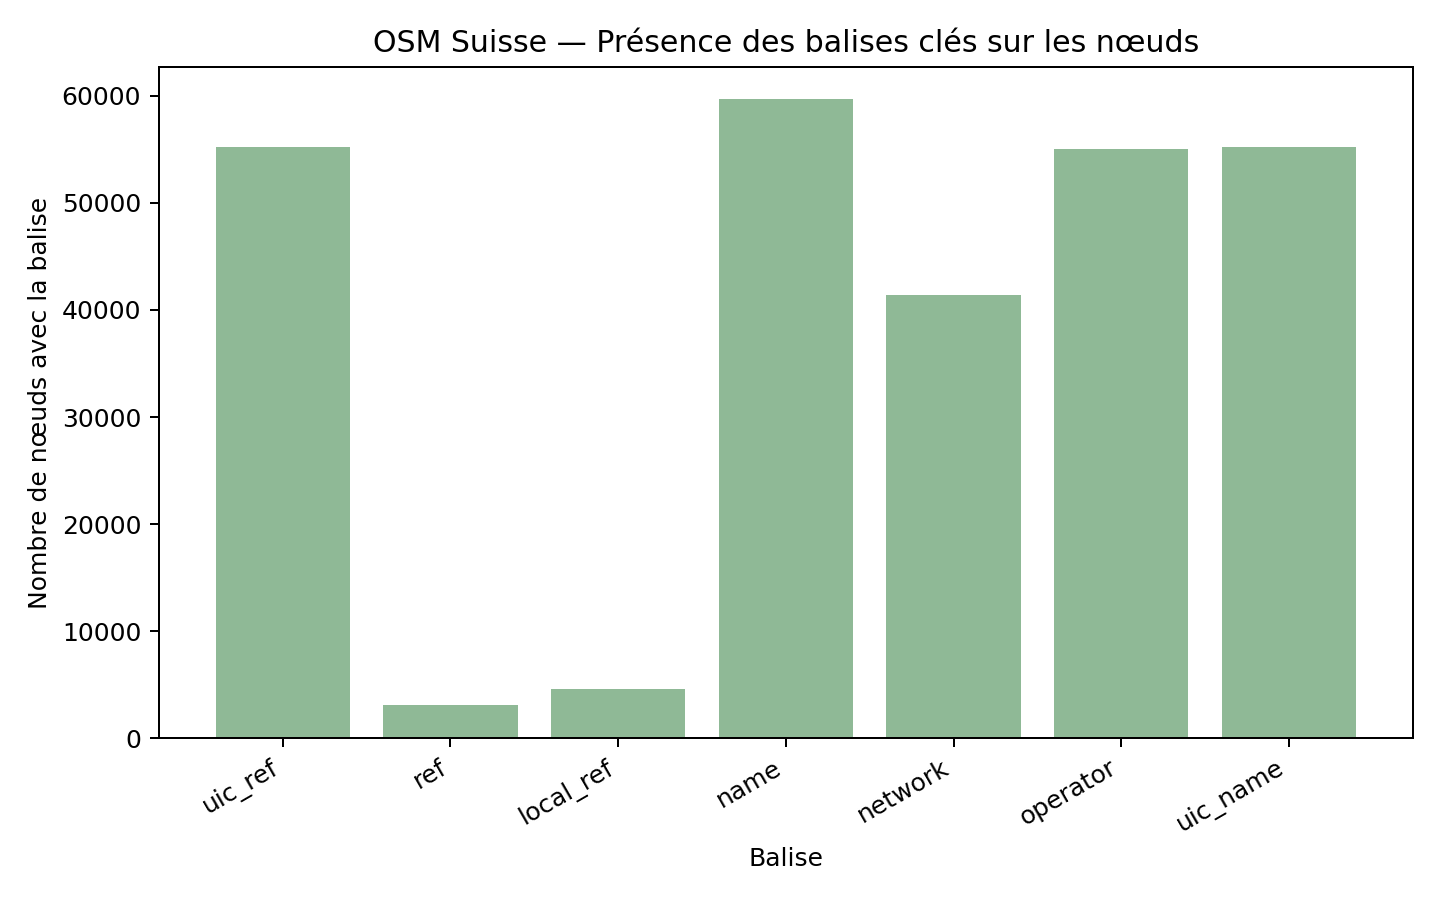
\includegraphics[width=.8\linewidth]{figures/plots/osm_tag_presence.png}
  \caption[Présence des balises clés]{Présence des balises clés par nœud (\texttt{uic\_ref}, \texttt{ref}, \texttt{local\_ref}, \texttt{name}, \texttt{network}, \texttt{operator}, \texttt{uic\_name}).}
  \label{fig:osm_tag_presence_inline}
\end{figure}

\section{Aperçu des itinéraires de transport public dans OSM en Suisse}

Comme mentionné dans le chapitre 1, nous nous intéressons également aux itinéraires, car ils peuvent nous aider à identifier des correspondances. Cela est particulièrement utile lorsqu'il existe deux arrêts pour une même station, mais pour des itinéraires empruntant des directions opposées, ou lorsque des arrêts de bus et de tram sont situés à proximité.

Voici quelques statistiques essentielles :

\begin{itemize}
    \item Total d'itinéraires uniques : 1 904  
    \item Total de connexions entre nœuds et itinéraires : 138 761  
    \item Nombre de nœuds desservant au moins un itinéraire : 51 286  
    \item Nombre moyen d'itinéraires par nœud : 2,71  
\end{itemize}

\begin{figure}[H]
  \centering
  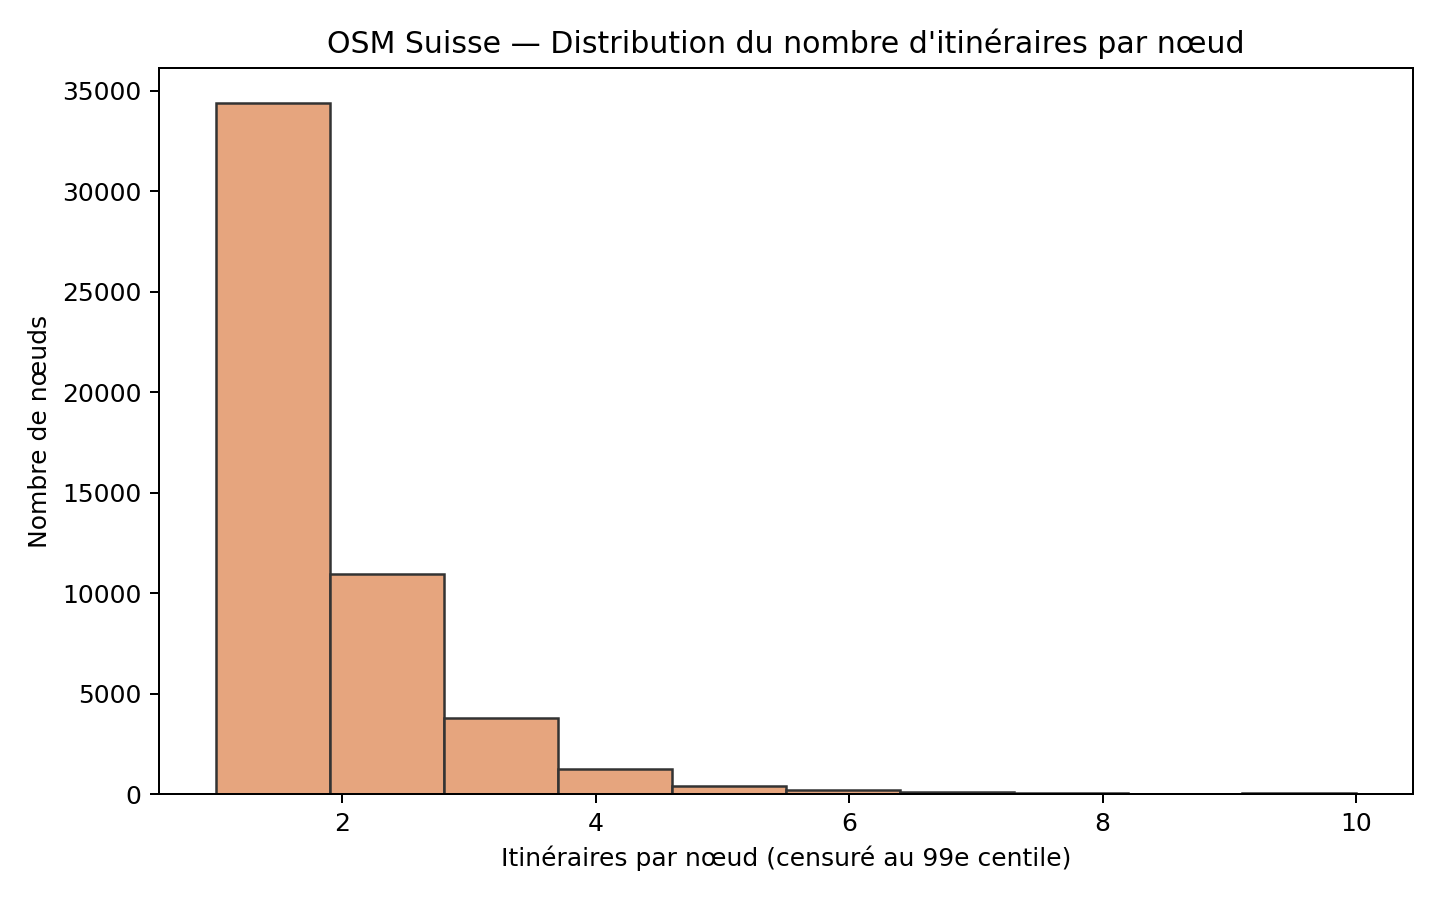
\includegraphics[width=.8\linewidth]{figures/plots/osm_routes_per_node_hist.png}
  \caption[Distribution des itinéraires par nœud]{OSM (Suisse) — distribution du nombre d'itinéraires distincts par nœud (censurée au 99e centile).}
  \label{fig:osm_routes_per_node_hist}
\end{figure}



\subsection{Les 5 nœuds de transport public les plus « connectés »}

\noindent\textit{Note méthodologique.} Cette liste est calculée en comptant le nombre de \textbf{connexions nœud–itinéraire} présentes dans le fichier \texttt{data/processed/osm\_nodes\_with\_routes.csv} (une ligne par appartenance d’un nœud à une relation OSM de type \texttt{route}). Il s’agit donc d’un \textbf{compte brut des relations} (directions et variantes incluses), et non d’un décompte de lignes distinctes après déduplication par \texttt{gtfs:route\_id}. Le script minimal reproduisant ce calcul est fourni sous \texttt{memoire/scripts\_used/chap2/compute\_busiest\_nodes.py}.

\begin{tcolorbox}[colback=blue!5, colframe=blue!40, title=\textbf{1er} — Zürich Bus Station, fontupper=\normalsize\bfseries]
\textbf{Itinéraires desservis :} 65 \\
\textbf{Type de nœud :} \texttt{stop\_position} \\
\textbf{Node ID :} 5962551000
\end{tcolorbox}

\begin{tcolorbox}[colback=green!5, colframe=green!40, title=\textbf{2e} — Stein, fontupper=\normalsize\bfseries]
\textbf{Itinéraires desservis :} 40 \\
\textbf{Type de nœud :} \texttt{stop\_position} \\
\textbf{Référence UIC :} 8580638 \\
\textbf{Node ID :} 984028248
\end{tcolorbox}

\begin{tcolorbox}[colback=orange!5, colframe=orange!40, title=\textbf{3e} — Genève - Gare Routière, fontupper=\normalsize\bfseries]
\textbf{Itinéraires desservis :} 37 \\
\textbf{Type de nœud :} \texttt{stop\_position} \\
\textbf{Node ID :} 960890428
\end{tcolorbox}

\begin{tcolorbox}[colback=purple!5, colframe=purple!40, title=\textbf{4e} — Lugano Centrale, fontupper=\normalsize\bfseries]
\textbf{Itinéraires desservis :} 37 \\
\textbf{Type de nœud :} \texttt{stop\_position} \\
\textbf{Référence UIC :} 8505550 \\
\textbf{Node ID :} 984002736
\end{tcolorbox}

\begin{tcolorbox}[colback=red!5, colframe=red!40, title=\textbf{5e} — Paradiso, fontupper=\normalsize\bfseries]
\textbf{Itinéraires desservis :} 34 \\
\textbf{Type de nœud :} \texttt{stop\_position} \\
\textbf{Référence UIC :} 8505553 \\
\textbf{Node ID :} 1266983076
\end{tcolorbox}

\subsection{Analyse des directions des itinéraires}

\begin{itemize}
    \item Direction 0 (généralement sortante) : 60 319 connexions  
    \item Direction 1 (généralement entrante) : 57 057 connexions  
    \item Direction inconnue : 21 385 connexions  
\end{itemize}

\begin{figure}[H]
  \centering
  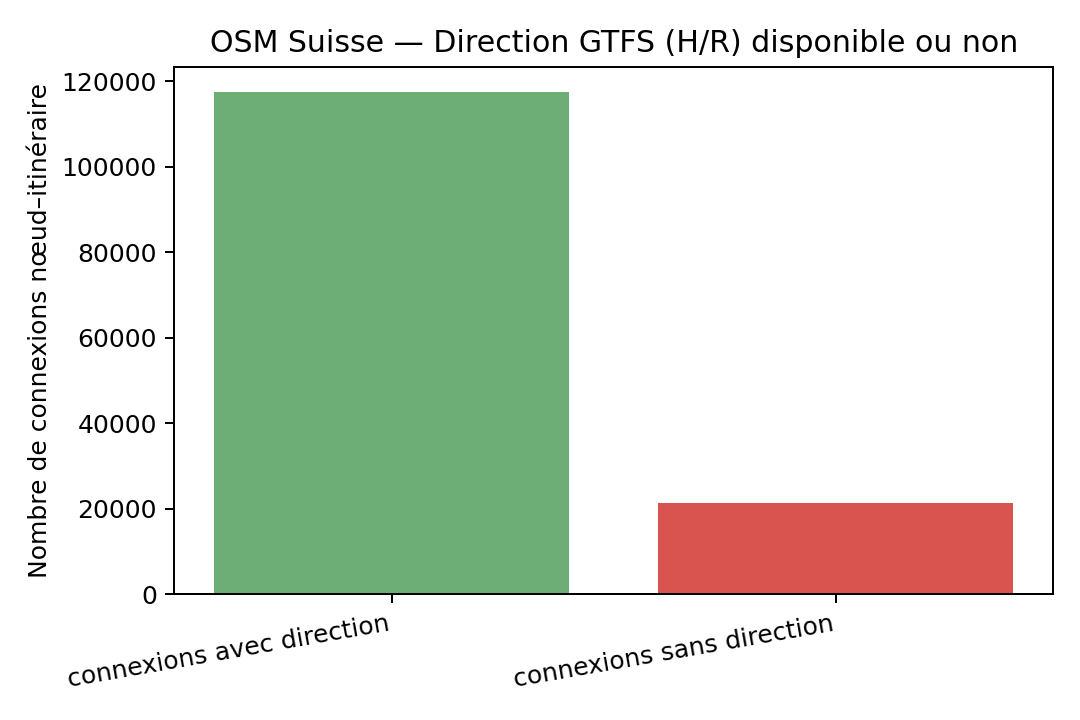
\includegraphics[width=.6\linewidth]{figures/plots/osm_direction_known_ratio.png}
  \caption[Directions H/R connues]{Connexions nœud–itinéraire pour lesquelles une direction (H/R) est déduite à partir de \texttt{ref\_trips}.}
  \label{fig:osm_direction_known_ratio_inline}
\end{figure}


\subsection{Top 5 des itinéraires avec le plus d’arrêts}

\begin{itemize}
    \item Bus 120 : Engelburg $\rightarrow$ St. Gallen $\rightarrow$ Eggersriet $\rightarrow$ Heiden : 174 arrêts  
    \item Bus 120 : Heiden $\rightarrow$ Eggersriet $\rightarrow$ St. Gallen $\rightarrow$ Engelburg : 174 arrêts  
    \item Bus 722 : Weinfelden $\rightarrow$ Hosenruck $\rightarrow$ Wil SG : 150 arrêts  
    \item Bus 722 : Wil SG $\rightarrow$ Hosenruck $\rightarrow$ Weinfelden : 150 arrêts  
    \item Bus 507 : Lostorf $\rightarrow$ Olten $\rightarrow$ Egerkingen : 138 arrêts  
\end{itemize}


